%% LaTeXTutorial.tex
%% Raj Kunamaneni
%% This file is meant to introduce how to get started on Latex for a new user.
%% ---------------------------------------------------------------------------------------------------
\documentclass[12pt,journal,compsoc]{IEEEtran}

%-----PACKAGES-------------------------------------------------------------------------------------
\usepackage{graphicx}

%----- The DOCUMENT Environment-------------------------------------------------------------------

\begin{document}

\title{Learning \LaTeX}
\author{Raj Kunamaneni}


% The paper headers
\markboth{\LaTeX\ IEEE Intro to Latex}%
{Kunamaneni \MakeLowercase{\textit{et al.}}: Tutorial}

\maketitle

%----- The SECTION Environment -------------------------------------------------------------------

\section{Introduction}

Latex is a tool that has been in use in academia since the early 80s and continues to be used. Presenting mathematical results or data efficiently are some of the benefits of using Latex in research and publication. Often the academia presents data via Latex which is widely used for scientific documents and other publishing material. Now you may be asking, why should I know to use Latex or even use it? Let me give you a personal example. The use of Latex has been very helpful to talk about the efficiency of my programs for example in CSE13S. Presenting material regarding the efficiency of different sorting methods and the corresponding graphs based on its time sorting large number set. By presenting mathematical data and results via Latex, the explanation process made it understandable to the reader and easier to put together complex equations which would be tougher to do on a regular word processor. This tool is imperative to know not only if you want to continue into research but will also be helpful in the industry. Now you understand the reasons. Let us get started.
 
\section{Creating a .tex file}

This section will cover the basics of creating a .tex file and libraries need to get started.

\subsubsection{Creating a Space}
Before we input any text, we need to include the type of appearance that we want our file to look like. For example, this file is using 

\begin{verbatim} \documentclass{IEEEtran} \end{verbatim}

\noindent When you create a file, try testing it out with different appearances and test which appearance you like to work with. To start inputting text to our document, you need to initialize the space of where the document begins \begin{verbatim} \begin{document} \end{verbatim}
and where it ends \begin{verbatim} \end{document} \end{verbatim} In general the \begin{verbatim} \begin{} and \end{} \end{verbatim} are used in LaTeX to show where the environment input starts and ends. This will create a space where you, the writer, will input data and results and the compiler will output the results to a expected output file type.

% Creating a subsubsection:

\subsubsection{Reserved Characters}
\begin{center}
 \textbackslash \ \ \~{} \ \ \textbackslash \textbackslash \ \ \%{}\\
\end{center}

What are Reserved Characters? These characters are used to serve a different purpose such as output and other purposes. For example the \textbackslash \  character provides that we are using a Latex command. For example if the user types \begin{verbatim} \LaTeX \end{verbatim} the output result will be \LaTeX. The \~{}  provides a non breakable space when inputting a large paragraph. This is used so it doesn't break the continuity of the sentence. The \ \textbackslash \textbackslash \ provide a new line to a paragraph or sentence. Finally, the  \%{}\ is the comment character. 

\subsubsection{Title and Heading}

It is important to include who is writing this article and when this article was created. For example this file uses

\begin{verbatim}
\title{Learning \LaTeX} 

\author{Raj Kunamaneni} 

\date{} 
\end{verbatim}

This part of creating the file is fairly self explanatory but in order to get today's current date we input \begin{verbatim} \today \end{verbatim} inside of the curly bracket of data. If we wanted January 1st, 2022 then we input \begin{verbatim} \date{January 1st, 2022} \end{verbatim} Finally, make title creates a separate title on different page other than the first or main page. This is helpful to introduce a new concepts in a document or another section of the paper if you were to do a research paper. \begin{verbatim} \maketitle \end{verbatim}

%----- Additional Features -----------------------------------------------------------------------

\section{Sections and Body Text}
Throughout this article you will see the use of sections and subsections. For example the bolded title above \textbf{3  Section} is a section. To create a section, we do \begin{verbatim} \section{Sections} \end{verbatim} 

\subsection{Subsection} 
The subsection is used for sub titles for the main section. An example to create a subsection would be to do \begin{verbatim} \subsubsection{Subsection} \end{verbatim}

\subsection{Body Text}
To create a paragraph just start typing and test it out via the output of the document. Some tools to use are \begin{verbatim} \parindent and \parskip \end{verbatim} The parindent creates an indent before the paragraph and creates spaces before the starting the actual content of the paragraph.

\section{Tables}
Tables are useful to present data. Such data for example would include addressing the results of Covid Result per state in the US. Let's not get too technical. First off let's create a table.

\begin{table}[h]
%% increase table row spacing, adjust to taste
\renewcommand{\arraystretch}{2.5}
% if using array.sty, it might be a good idea to tweak the value of
%\extrarowheight as needed to properly center the text within the cells
\caption{Table of Pets}
\label{table_example}
\centering
%% Some packages, such as MDW tools, offer better commands for making tables
%% than the plain LaTeX2e tabular which is used here.
\begin{tabular}{|c|c|}
\hline
Dog & Cat\\
\hline
Rabbit & Mouse\\
\hline
\end{tabular}
\end{table}

The table above will be used by the \\commands 

\begin{verbatim} \begin{table} \end{verbatim} and to end the table do \begin{verbatim} \end{table} \end{verbatim}

\noindent This creates a simple table but how do we fill in the contents of the table? We use the tabular command to do so. First 

\begin{table}[h]
\renewcommand{\arraystretch}{1.5}
\caption{Table of Animals}
\centering
\begin{tabular}{|c||c||c|}
\hline
Dog & Cat & Kitten\\
\hline
Dog & Cat & Dog\\
\hline
\end{tabular}
\end{table}

\begin{verbatim} \begin{tabular}{|c||c||c|} \end{verbatim} and to end the tabular environment for table do \begin{verbatim} \end{tabular} \end{verbatim} You may be asking what is the \begin{verbatim} |c||c||c| \end{verbatim} 

The c is for centered column. If you want the text to be centered use this command. Some other helpful things to know: r for right justified column, l for left-justified column, $|$ \ is a vertical line which is used for distinguishing the table in sub groups (check out Table 1), and $||$ \ is a \\double vertical line which has a similar purpose to $|$ \ but it clearly distinguishes between the contents of the table. An example would be Table 2 above. In order to fill contents of the table, we use the 

\begin{verbatim}
\hline
\end{verbatim} command to do so. An example from Table 2 would be 

\begin{verbatim} 
\hline
Dog & Cat & Kitten
\end{verbatim}

\noindent This will fill in the first column and the \textbackslash \textbackslash \ creates a newline or moves to the next row. This is the simplicity and beauty of creating tables in LaTeX. 

\section{Figures}

In any document it is important to include a picture corresponding to your result in your data or a simple picture. The question is how do we do it in LaTeX?

\begin{figure}[h] 	% There are several different modifiers that can be used in [].
\centering

\includegraphics[width=2in]{UCSClogo.png}
\caption{Sammy the Slug}
\label{fig_slug}
\end{figure}

\noindent First off in LaTeX, it needs to have a picture in the same directory as the .tex file. Next we create 

\begin{verbatim}
\begin{figure}

\end{figure}
\end{verbatim}

\noindent Inside the statements we call 

\begin{verbatim}
\includegraphics[]{}
\end{verbatim}

\noindent Inside the bracket, include the dimensions of the picture and inside the curly brackets you include the picture that you want in your document. Below the picture, you would see a caption explaining the context of the photo. To do this in LaTeX do 

\begin{verbatim}
\caption{Sammy the Slug}
\end{verbatim}

What about when you would want to include data from a Lab Experiment? Lets include at Titration Plot and the corresponding data. 

\begin{figure}[h] 	% There are several different modifiers that can be used in [].
\centering
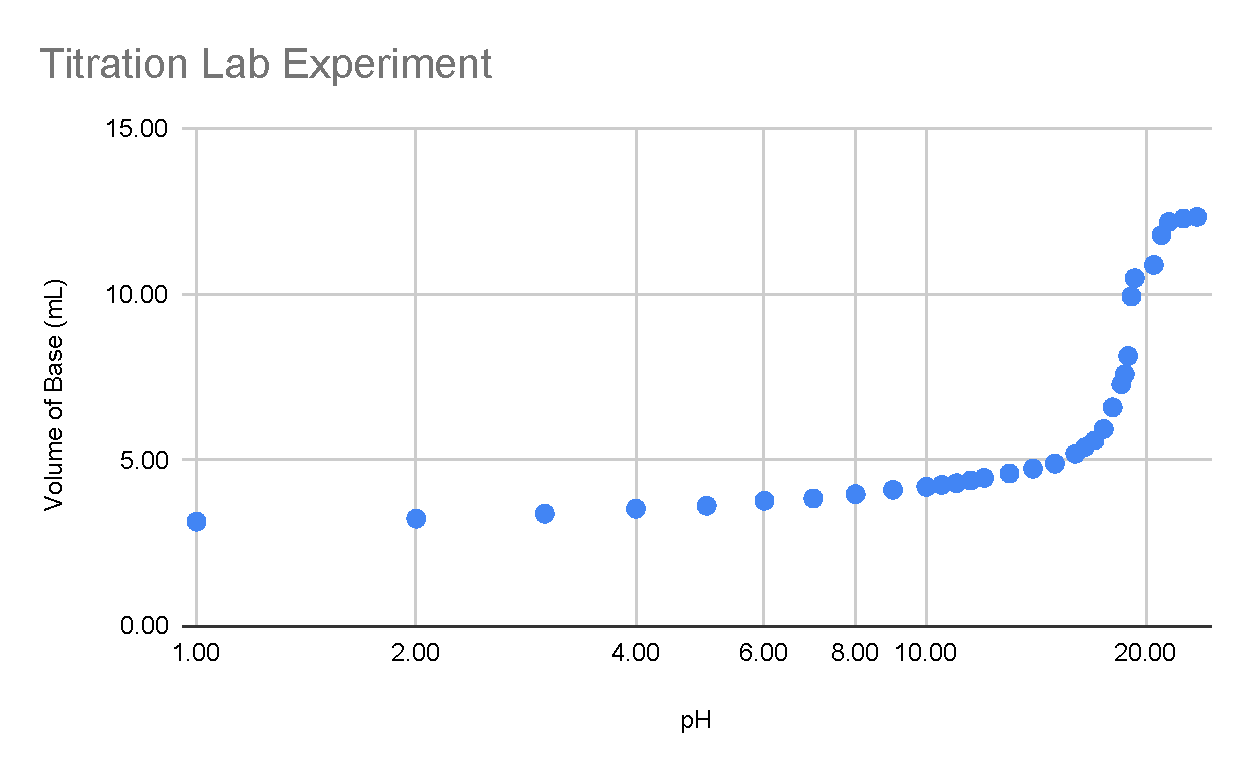
\includegraphics[width=3.8in]{Titration Lab Experiment.pdf}
\caption{Titration Plot}
\label{fig_plot}
\end{figure}

and the graph is calculated from the following data

\begin{figure}[h] 	% There are several different modifiers that can be used in [].
\centering
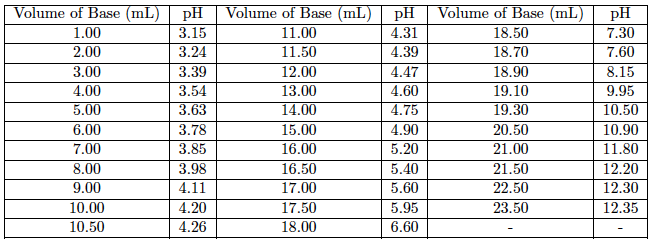
\includegraphics[width=3.8in]{Data.png} 
\caption{Titration Plot Data}
\label{fig_plot}
\end{figure}

The purpose of this is to show that this can be applicable to feature data for research papers and displaying results. 

\section{Mathematical Formulas}

There are multiple operations for creating Mathematical Formulas in LaTeX but this introduction will touch upon the important concepts that will help get you started. 

\noindent \\\\\\   Using the 
\begin{verbatim}
\begin{equation} 

E = {m * c^2}

\end{equation}
\end{verbatim}

Will display a equation. For example:

\begin{equation}
    E = {m * c^2} 
\end{equation}

\noindent Another way would be to do a in-line expression such as $E = {m * c^2}$. To this, use the double dollar sign and insert the equation inside. Example below. 

\begin{verbatim}
$ E = {m * c^2} $
\end{verbatim}

The equation can be used in any context such as Matrix or other mathematical expression. Would highly recommend reading the \textbf{www.overleaf.com/learn} about more uses of Mathematical Expressions and other interesting features. To create symbols in Latex for expressions, like this $\int$ or $\sqrt{40}$. Type in the \textbackslash  and input a symbol for an expression.

\begin{verbatim}
\int 
or
\sqrt{numbers}
\end{verbatim}

\noindent Next, we are going to be talking about fractions in LaTeX. To do, $\frac{2}{3}$ do 
\begin{verbatim}
$\frac{2}{3}$ 
\end{verbatim}
\noindent The first bracket is where you input the numerator value and in the second bracket, you input the denominator value. Finally, let us talk about how to do a superscript and subscript, this is a superscript or a exponent $ 4^{2} = 16 $ and the following is a subscript $ Y_{3} $. 

\begin{verbatim}
$ 4^{2} = 16 $ <-- superscript
$ Y_{3} $      <-- subscript
\end{verbatim}

\noindent Using the dollar signs makes it simple to create an in-line for the super and subscript. 

\section{Acknowledgement}

The Acknowledgement section is where you introduce anyone or the source that you referenced in a paper. For example, a reference would be Michael Shell as they created the CLS for the this document. This is important as you always want to give credit for the people who help contribute to your project. Check the example in the end of the paper. 

\section{References}

The References section give credit to any resources or pictures that you referenced throughout your LaTeX document. Use command such as:

\begin{verbatim} \label{fig_slug} \end{verbatim}
\noindent This will create a label for your picture or graph. Reference the object throughout this document. 

\begin{verbatim} \ref{fig_slug} \end{verbatim} appears like: \ref{fig_slug}\\
\noindent This creates a reference or citation of where this was used from. 

\begin{verbatim} \cite{IEEEhowto:kopka} \end{verbatim} 
Finally, you would want to use a cite to reference the sources you got your information or data from. This will create a number that can be accessed at the end of the document, where you can see the context behind that citation. 

Lastly, in your reference you would want to include a Bibliography page on your citations. To start this you need 
\begin{verbatim} 
\begin{thebibliography}
and 
\end{thebibliography}\end{verbatim} 
This is where you include all the full citations with the authors and the publication. Examples will be below for your viewing. Using the \begin{verbatim} \bibitem \end{verbatim} will reference the information that you are using. 

\section{Conclusion}
This document hopefully gives you an introduction to LaTeX and the values of why this is a powerful software to use. I recommend reading the sources below as there are cheat sheets that make it faster for you to get started and bring out your best in your future research projects. If you want a better understanding of how to get started, download the .tex file, and feel free to edit this document and play around with it to get comfortable with LaTeX. Good Luck on your journey in LaTeX. 


%----- BIBLIOGRAPHY ------------------------------------------------------------------------------
%Cite: https://www.overleaf.com/learn/latex/Learn_LaTeX_in_30_minutes?&nocdn=true#What_is_LaTeX.3F
%https://www.giss.nasa.gov/tools/latex/ltx-164.html
%Titration Plot (need to include)
%https://www.dickimaw-books.com/latex/novices/html/symbols.html
%https://www.bu.edu/math/files/2013/08/LongTeX1.pdf
%https://d1b10bmlvqabco.cloudfront.net/attach/isozumojo0o1ko/isp2cy0py1t5de/iu492uz43t93/Introduction_to_latex.pdf
%http://latexref.xyz/Reserved-characters.html
%https://www.giss.nasa.gov/tools/latex/ltx-263.html
%https://d1b10bmlvqabco.cloudfront.net/attach/isozumojo0o1ko/isp2cy0py1t5de/iu492uz43t93/Introduction_to_latex.pdf
%ucsc logo from: https://en.wikipedia.org/wiki/UC_Santa_Cruz_Banana_Slugs#/media/File:SDS_UCSantaCruz_RedwoodSlug_WhiteGround.png

\begin{thebibliography}{1}
\bibitem[Intro To Latex OverLeaf] 
\url{www.overleaf.com/learn/latex}

\bibitem[NASA LaTeX Tools] 
\url{www.giss.nasa.gov/tools/latex}

\bibitem[Dickimaw Books] 
\url{www.dickimaw-books.com/latex/novices/html/symbols.html}

\bibitem[LaTeX Reference] 
\url{www.latexref.xyz/Reserved-characters.html}

\bibitem[Slug Logo] 
\url{https://news.ucsc.edu/2020/06/new-strong-slug.html}

\bibitem[Titration Plot Data] 
\url{https://cse185e-spring22-01.courses.soe.ucsc.edu/home}

\end{thebibliography}

\end{document}